\documentclass[journal,12pt,twocolumn]{IEEEtran}

\usepackage{setspace}
\usepackage{gensymb}
\singlespacing
\usepackage[cmex10]{amsmath}

\usepackage{amsthm}

\usepackage{mathrsfs}
\usepackage{txfonts}
\usepackage{stfloats}
\usepackage{bm}
\usepackage{cite}
\usepackage{cases}
\usepackage{subfig}

\usepackage{longtable}
\usepackage{multirow}

\usepackage{enumitem}
\usepackage{mathtools}
\usepackage{steinmetz}
\usepackage{tikz}
\usepackage{circuitikz}
\usepackage{verbatim}
\usepackage{tfrupee}
\usepackage[breaklinks=true]{hyperref}
\usepackage{graphicx}
\usepackage{tkz-euclide}

\usetikzlibrary{calc,math}
\usepackage{listings}
    \usepackage{color}                                            %%
    \usepackage{array}                                            %%
    \usepackage{longtable}                                        %%
    \usepackage{calc}                                             %%
    \usepackage{multirow}                                         %%
    \usepackage{hhline}                                           %%
    \usepackage{ifthen}                                           %%
    \usepackage{lscape}     
\usepackage{multicol}
\usepackage{chngcntr}

\DeclareMathOperator*{\Res}{Res}

\renewcommand\thesection{\arabic{section}}
\renewcommand\thesubsection{\thesection.\arabic{subsection}}
\renewcommand\thesubsubsection{\thesubsection.\arabic{subsubsection}}

\renewcommand\thesectiondis{\arabic{section}}
\renewcommand\thesubsectiondis{\thesectiondis.\arabic{subsection}}
\renewcommand\thesubsubsectiondis{\thesubsectiondis.\arabic{subsubsection}}


\hyphenation{op-tical net-works semi-conduc-tor}
\def\inputGnumericTable{}                                 %%

\lstset{
%language=C,
frame=single, 
breaklines=true,
columns=fullflexible
}
\begin{document}


\newtheorem{theorem}{Theorem}[section]
\newtheorem{problem}{Problem}
\newtheorem{proposition}{Proposition}[section]
\newtheorem{lemma}{Lemma}[section]
\newtheorem{corollary}[theorem]{Corollary}
\newtheorem{example}{Example}[section]
\newtheorem{definition}[problem]{Definition}

\newcommand{\BEQA}{\begin{eqnarray}}
\newcommand{\EEQA}{\end{eqnarray}}
\newcommand{\define}{\stackrel{\triangle}{=}}
\bibliographystyle{IEEEtran}
\raggedbottom
\setlength{\parindent}{0pt}
\providecommand{\mbf}{\mathbf}
\providecommand{\pr}[1]{\ensuremath{\Pr\left(#1\right)}}
\providecommand{\qfunc}[1]{\ensuremath{Q\left(#1\right)}}
\providecommand{\sbrak}[1]{\ensuremath{{}\left[#1\right]}}
\providecommand{\lsbrak}[1]{\ensuremath{{}\left[#1\right.}}
\providecommand{\rsbrak}[1]{\ensuremath{{}\left.#1\right]}}
\providecommand{\brak}[1]{\ensuremath{\left(#1\right)}}
\providecommand{\lbrak}[1]{\ensuremath{\left(#1\right.}}
\providecommand{\rbrak}[1]{\ensuremath{\left.#1\right)}}
\providecommand{\cbrak}[1]{\ensuremath{\left\{#1\right\}}}
\providecommand{\lcbrak}[1]{\ensuremath{\left\{#1\right.}}
\providecommand{\rcbrak}[1]{\ensuremath{\left.#1\right\}}}
\theoremstyle{remark}
\newtheorem{rem}{Remark}
\newcommand{\sgn}{\mathop{\mathrm{sgn}}}
\providecommand{\abs}[1]{\left\vert#1\right\vert}
\providecommand{\res}[1]{\Res\displaylimits_{#1}} 
\providecommand{\norm}[1]{\left\lVert#1\right\rVert}
%\providecommand{\norm}[1]{\lVert#1\rVert}
\providecommand{\mtx}[1]{\mathbf{#1}}
\providecommand{\mean}[1]{E\left[ #1 \right]}
\providecommand{\fourier}{\overset{\mathcal{F}}{ \rightleftharpoons}}
%\providecommand{\hilbert}{\overset{\mathcal{H}}{ \rightleftharpoons}}
\providecommand{\system}{\overset{\mathcal{H}}{ \longleftrightarrow}}
	%\newcommand{\solution}[2]{\textbf{Solution:}{#1}}
\newcommand{\solution}{\noindent \textbf{Solution: }}
\newcommand{\cosec}{\,\text{cosec}\,}
\providecommand{\dec}[2]{\ensuremath{\overset{#1}{\underset{#2}{\gtrless}}}}
\newcommand{\myvec}[1]{\ensuremath{\begin{pmatrix}#1\end{pmatrix}}}
\newcommand{\mydet}[1]{\ensuremath{\begin{vmatrix}#1\end{vmatrix}}}
\numberwithin{equation}{subsection}
\makeatletter
\@addtoreset{figure}{problem}
\makeatother
\let\StandardTheFigure\thefigure
\let\vec\mathbf
\renewcommand{\thefigure}{\theproblem}
\def\putbox#1#2#3{\makebox[0in][l]{\makebox[#1][l]{}\raisebox{\baselineskip}[0in][0in]{\raisebox{#2}[0in][0in]{#3}}}}
     \def\rightbox#1{\makebox[0in][r]{#1}}
     \def\centbox#1{\makebox[0in]{#1}}
     \def\topbox#1{\raisebox{-\baselineskip}[0in][0in]{#1}}
     \def\midbox#1{\raisebox{-0.5\baselineskip}[0in][0in]{#1}}
\vspace{3cm}
\title{AI5002: Assignment 8}
\author{Debolena Basak\\ AI20RESCH11003}
\maketitle
\newpage
\bigskip
\renewcommand{\thefigure}{\theenumi}
\renewcommand{\thetable}{\theenumi}
Download all Python codes from 
\begin{lstlisting}
https://github.com/Debolena/AI5002-Probability-and-Random-Variables/blob/main/Assignment_8/python_assignment_8.py
\end{lstlisting}
%
and latex-tikz codes from 
%
\begin{lstlisting}
https://github.com/Debolena/AI5002-Probability-and-Random-Variables/blob/main/Assignment_8/latex.tex
\end{lstlisting}
\section{Problem}
Let X denote the number of hours you study
during a randomly selected school day. The
probability that X can take the values x, has
the following form, where k is some unknown
constant.\\
\begin{align}
    P\brak{X=x} =
    \begin{cases}
      0.1, & \text{if}\ x=0 \\
      kx,  & \text{if}\ x= 1 \; \text{or}\ 2 \\
      k(5-x) & \text{if}\ x= 3 \; \text{or}\ 4 \\
      0, & \text{otherwise}
    \end{cases}
  \end{align}
\begin{enumerate}
    \item Find the value of k.
    \item What is the probability that you study at
least two hours ? Exactly two hours? At most
two hours?
\end{enumerate}
\section{Solution}
1)
We know, sum of the all probabilities $= 1$
\begin{align}
    & \quad \sum_{x=0}^4 P(X=x) = 1\\
    &\implies 0.1 + k +2k +2k +k = 1\\
    &\implies 0.1 +6k = 1\\
    &\implies k = 0.15
\end{align}
2)
Probability of studying atleast 2 hours
\begin{align}
    &= P\brak{X\ge 2}\\
    &=\sum_{x=2}^4 P(X=x)\\
    &= P(X=2)+ P(X=3) +P(X=4)\\
    &= 2k + 2k +k\\
    &= 5* 0.15\\
    &= 0.75
\end{align}
Probability of studying exactly 2 hours
\begin{align}
    &=P(X=2)\\
    &= 0.15* 2\\
    &= 0.30
\end{align}
Probability of studying atmost 2 hours
\begin{align}
    &= P\brak{X\le 2}\\ 
    &=\sum_{x=0}^2 P(X=x)\\
    &= P(X=0) + P(X=1)+ P(X=2)\\
    &= 0.1 + 0.15 +0.30\\
    &=0.55
\end{align}
NOTE:\\
Suppose A= event of studying atleast 2 hours\\
B= event of studying atmost 2 hours\\
Then clearly, $A \cap B$ is the event of studing exactly two hours.\\
We can verify here that
\begin{align}
    &P(A) + P(B) -P(A \cap B) \\
    &= 0.75 +0.55 - 0.30 \\
    &=1
\end{align}
\begin{figure}[!ht]
\centering
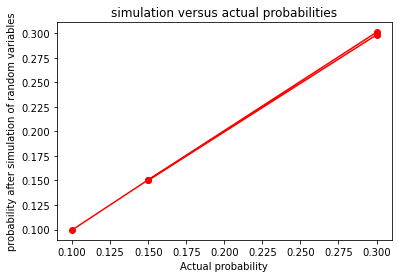
\includegraphics[width=\columnwidth]{actual_vs_simulated plot.png}
\caption{Actual Vs Simulated Plot}
\label{fig:Actual Vs Simulated Plot}
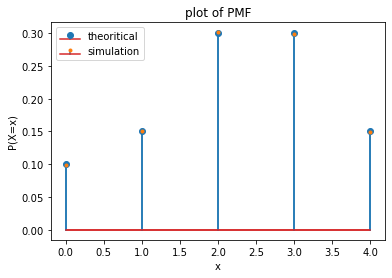
\includegraphics[width=\columnwidth]{pmf plot.png}
\caption{PMF Plot}
\label{fig:PMF Plot}
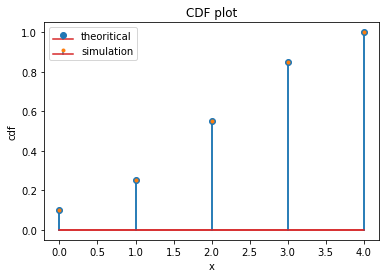
\includegraphics[width=\columnwidth]{cdf plot.png}
\caption{CDF Plot}
\label{fig:CDF Plot}
\end{figure}
\end{document}
